\chapter{Linear Regression}

\section{Notation}

In general we format variables as: $x$ for scalars, $\x$ for vectors, and $X$ for matrices.
\begin{itemize}
  \item Input / Feature space / Attributes Space :  \(\mathcal{X} =  \mathbb{R}^d\) for some \(d\in\mathbb{N}\)
  \item Output / \emph{Label space} / Response space : \( \mathcal{Y}= \mathbb{R} \)
  \item Dataset : \( \D = \left\{(\tc{x}_i,y_i)\right\}_{i=1}^{n} \), where \(\tc{x}_i \in \mathcal{X}, y_i \in \mathcal{Y} \ \forall \ i \in \{1\ldots n\}\)
\end{itemize}

We consider a target function $f : \mathcal{X} \to \mathcal{Y}$ on the training dataset $\D$, i.e. $\tc{x} \overset{f}{\mapsto} y \ \forall \ (\x,y) \in \D$. \\

We focus on the task of finding a \emph{hypothesis function} \(h : \mathcal{X} \to \mathcal{Y}\) that ideally closely approximates \(f\). We call the family of the hypothesis functions as \(\mathcal{H}\), the \emph{Hypothesis Class}. It follows that \(h \in \mathcal{H}\)
This now brings the following questions:
\begin{enumerate}
  \item What are the possibilities for the predictor function \(h\) ? [\tc{Hypothesis Class}]
  \item How do you quantify the performance of the predictor? [\tc{Loss/Error Function}]
  \item How do we find the best predictor? [\tc{Optimization}]
\end{enumerate}

\section{What are the possible predictor functions?}

Let us first play with a simpler case with a one-dimensional feature space. We may consider the problem as a line fitting problem, taking our hypothesis class to be all linear functions.

\begin{figure}[H]
  \centering
  \begin{tikzpicture}
    \begin{axis}[
        axis lines=middle,
        xlabel=$x$,
        ylabel=$y$,
        xmin=0, xmax=10,
        ymin=0, ymax=15,
        xtick={0,2,...,5},
        ytick={0,3,...,9},
        grid=both,
        grid style={line width=0.1pt, draw=gray!30},
      ]
      \addplot[only marks, mark=*, blue] coordinates {
          (1, 2)
          (2, 4)
          (3, 5)
          (4, 7)
          (5, 8)
          (2,9)
          (4,2)
          % Add more data points here
        };
      \addplot[red] {1.5*x + 0.5}; % Change the slope and intercept as needed
    \end{axis}
  \end{tikzpicture}
  \caption{Fitting a line to the data}
\end{figure}

Let us parametrize the line with $w_0,w_1$ (intercept and slope). We can vectorize our parameters as $W = \begin{bmatrix} w_0 \\ w_1 \end{bmatrix}$. Then we may write our hypothesis function $h_\w$ parametrised by $\w$ as.

$$
  h_\w(x) = w_0 + w_1 x
$$

Let us also vectorize our input as $\x = \begin{bmatrix} 1 \\ x \end{bmatrix}$, so that
$$
  h_{\w}(\x) = \tr{\w} \x
$$

We can now extend this to the multidimensional case. We consider our function to return a linear combination of our \(d\) dimensional features. \newline

\begin{figure} [h]
  \centering
  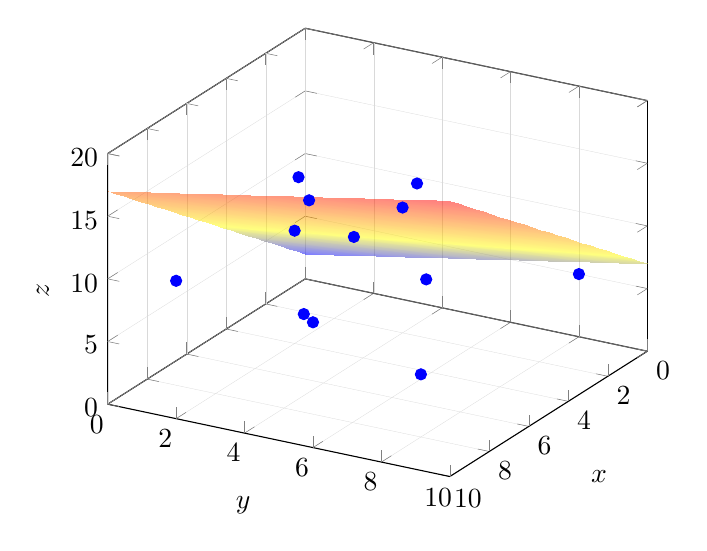
\begin{tikzpicture}
    \begin{axis}[
        view={120}{30},
        xlabel=$x$,
        ylabel=$y$,
        zlabel=$z$,
        xmin=0, xmax=10,
        ymin=0, ymax=10,
        zmin=0, zmax=20,
        xtick={0,2,...,10},
        ytick={0,2,...,10},
        ztick={0,5,...,20},
        grid=both,
        grid style={line width=0.1pt, draw=gray!30},
      ]

      \addplot3[only marks, mark=*, blue] coordinates {
          (0,8,5)
          (1, 2, 5.5)
          (2, 4, 10)
          (3, 5, 13.5)
          (4, 2, 9)
          (5, 3, 13)
          (6, 7, 10)
          (7, 4, 6.5)
          (8, 8, 5)
          (9, 5, 20)
          (10, 6, 10)
          (10, 2, 11)
        };

      \addplot3[
        surf,
        opacity=0.5,
        shader=interp,
        domain=0:10,
        domain y=0:10,
      ] {1.5*x + 0.5*y + 2}; % Adjust the coefficients as needed

    \end{axis}
  \end{tikzpicture}
  \caption{For higher dimensional feature spaces, linear regression is akin to \emph{Hyperplane Fitting}}
\end{figure}

We now have our parameter \(\w = \begin{bmatrix}w_0\\w_1\\\vdots\\w_d\end{bmatrix} \in \mathbb{R}^{d+1}\) and input vector \(\x = \begin{bmatrix}1\\x_1\\\vdots\\x_d\end{bmatrix}\) to get a identical expression -

$$
  h_\w(\x) = \tr{\w} \x
$$
Our hypothesis class is, then -
$$
  \mathcal{H} = \{ h_\w : \w \in \mathbb{R}^{d+1} \}
$$

This is essentially the \textit{linear} in linear regression. However, note that it does not mean we are restricted to linear functions of the features, we may transform the feature space to another space to regress.

\section{How to quantify the performance of a predictor ?}

We define a function that operates on the predictor function and dataset to quantify the "mismatch" between the two. Higher the loss function, lesser is the given predictor suitable for the dataset. Given that our function is parametrized, we may also define the loss function in terms of the parameter.

$$
  \text{Loss Function: } \loss(h,\D) ~\text{or}~ \loss(\w,\D)
$$

Let us consider a singleton dataset $\D_{test} =\{(\x,y)\}$ where $\x = \tr{\left[1~x_1~\ldots~x_d\right]}$. We define a loss for this dataset as
$$
  \loss(\w,\D_{test}) = (y-h_\w(\x))^2 = |y-\hat{y}|^2
$$

We define \(h_\w(x) = \hat{y}\), and \(|y-\hat{y}|\) is called a \emph{residual}. \\

Now for a dataset containing $n$ datapoints,

$$
  \mathbf{Least\ Squares\ Loss:} \ \  \loss(\w,\D_{train}) = \frac{1}{n} \sum_{i=1}^n(y_i-h_\w(\x_i))^2 = \frac{1}{n} \sum_{i=1}^n \left|y_i - \hat{y}_i\right|^2
$$

Note that the least squares loss is the mean of the squares of the residuals. We can also define a loss equal to the mean residual value.

$$
  \text{Mean Absolute Error Loss:} \ \ \loss({\w,\D_{train}}) = \frac{1}{n} \sum_{i=1}^n \left|y_i - \hat{y}_i\right|
$$

The Mean Absolute Error does not penalise high deviations as much as the Squares Loss, thus it may be more appropriate to use when the dataset contains many outliers.
\begin{figure}[htbp]
  \centering
  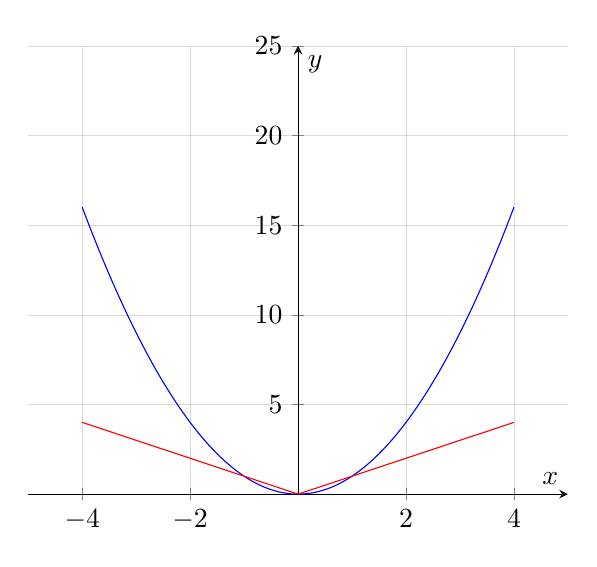
\begin{tikzpicture}
    \begin{axis}[
        axis lines=middle,
        xlabel=$x$,
        ylabel=$y$,
        xmin=-5, xmax=5,
        ymin=0, ymax=25,
        xtick={-4,-2,0,2,4},
        ytick={0,5,10,15,20,25},
        grid=both,
        grid style={line width=0.1pt, draw=gray!30},
      ]
      \addplot[blue, domain=-4:4, samples=100] {x^2};
      \addplot[red, domain=-4:4, samples=100] {abs(x)};
    \end{axis}
  \end{tikzpicture}
\end{figure}

Here we are interested in the least squares loss. We can vectorize the loss function as follows

$$
  \boxed{\mathbf{\loss(\w, \D_{\text{train}}) = \frac{1}{n} \lVert \y \mathrm{-} X\w \rVert_2^2}}
$$

$$
  \text{, where } X =
  \begin{bmatrix}
    \longleftarrow{\tr{\x_1}} \longrightarrow \\
    \longleftarrow \tr{\x_2} \longrightarrow  \\
    \vdots                                    \\
    \longleftarrow \tr{\x_n} \longrightarrow
  \end{bmatrix}_{n\times (d+1)}, \quad
  \y =
  \begin{bmatrix}
    y_1    \\
    y_2    \\
    \vdots \\
    y_n
  \end{bmatrix}_{n\times 1}\quad
$$

\section{How do we find the best predictor?}

We use the loss function to find our optimum hypothesis $h^*$, where
$$
  h^* = \argmin_{h \in \mathcal{H}} \loss(h,\D_{train})
$$

[Note that the optimisation is performed only over the training dataset]

We may also define the objective in terms of the parameter $\w$ corresponding to $h$.

\begin{align*}
  \w^*    & = \argmin_{\w} \loss(\w,\D_{train})            \\
  \w_{LS} & = \argmin_{\w} \sum_{i=1}^n(y_i-\tr{\w} x_i)^2
\end{align*}

We set out to find a closed form solution for \(\w_{LS}\) for $d$ dimensional data:

To find the optimum, we set the derivative\footnotemark[1] to zero. We may drop the \(\frac{1}{n}\) term.
\begin{align*}
  \nabla_\w\loss & = \frac{\partial{\loss(\w,\D_{train})}}{\partial{\w}} = \left[\frac{\partial{\loss(\w,\D_{train})}}{\partial{w_i}}\right]_{i=1}^n = \left[-2(y_i-\tr{\w} x_i)x_i\right]_{i=1}^n = 0 \\
  \implies       & 2(-\tr{X} \y + \tr{X} X\w) =0                                                                                                                                                       \\
  \implies       & \w_{LS} = (\tr{X} X)^{-1}\tr{X} Y
\end{align*}

We can also derive this result with vector-derivative identities\footnotemark[1],
\begin{align*}
           & \nabla_\w\loss = 0                                                                                                                                       \\
  \implies & \frac{\partial }{\partial \w} \lVert \y-X\w\rVert_2^2 = \frac{\partial}{\partial \w}\left(\tr{\y}\y - 2\tr{\w} \tr{X} \y + \tr{\w} \tr{X} X\w\right) = 0 \\
  \implies & -2\tr{X} \y + 2\tr{X}X\w = 0                                                                                                                             \\
  \implies & \tr{X}X\w = \tr{X}\y                                                                                                                                     \\
           & \boxed{\w = (\tr{X} X)^{-1}(\tr{X} \y)}
\end{align*}
Note that \(\tr{X}X\) need not be invertible.

\section{Homework}
For 1D data, $ h_\w(x)=w_0+w_1 x $,
prove that --
\begin{equation*}
  {\w_1}^* = \frac{\sum (x_i-\bar{x})(y_i-\bar{y})}{\sum (x_i-\bar{x})^2}
\end{equation*}

where \(\bar{x} = \frac{\sum{x_i}}{N} \text{ \ and \ } \bar{y} = \frac{\sum{y_i}}{N}\).

\begin{solution}
  \begin{align*}
    \mathcal{L}                               & = \sum_{i=1}^N (y_i-w_0-w_1x_i)^2                                                     \\
    \frac{\partial \mathcal{L}}{\partial w_0} & = - \sum_{i=1}^N (y_i-w_0-w_1x_i) = 0                                                 \\
    \implies  w_0^*                           & = \bar{y} - w_1\bar{x}                                                                \\
    \frac{\partial \mathcal{L}}{\partial w_1} & = - \sum_{i=1}^N x_i(y_i-w_0-w_1x_i) = 0                                              \\
    \implies w_1^*                            & = \frac{\sum_{i=1}^N x_iy_i - Nw_0^*\bar{x}} {\sum_{i=1}^N x_i^2}                     \\
                                              & = \frac{\sum_{i=1}^N x_iy_i - N\bar{x}\bar{y} + w_1^*N\bar{x}^2} {\sum_{i=1}^N x_i^2} \\
                                              & = \frac{\sum_{i=1}^N (x_iy_i - \bar{x}\bar{y})} {\sum_{i=1}^N (x_i-\bar{x})^2}        \\
                                              & = \frac{\sum_{i=1}^N (x_i-\bar{x})(y_i-\bar{y})} {\sum_{i=1}^N (x_i-\bar{x})^2}
  \end{align*}
\end{solution}

\footnotetext[1]{There are two conventions for the derivative of a scalar by a vector, i.e., whether the result is a \href{https://www.cs.huji.ac.il/w~csip/tirgul3_derivatives.pdf}{row} or \href{https://onlinelibrary.wiley.com/doi/pdf/10.1002/0471705195.app3}{column}. Here we will stick with the latter.}

\newpage
\section{Basis Functions}

\begin{center}
  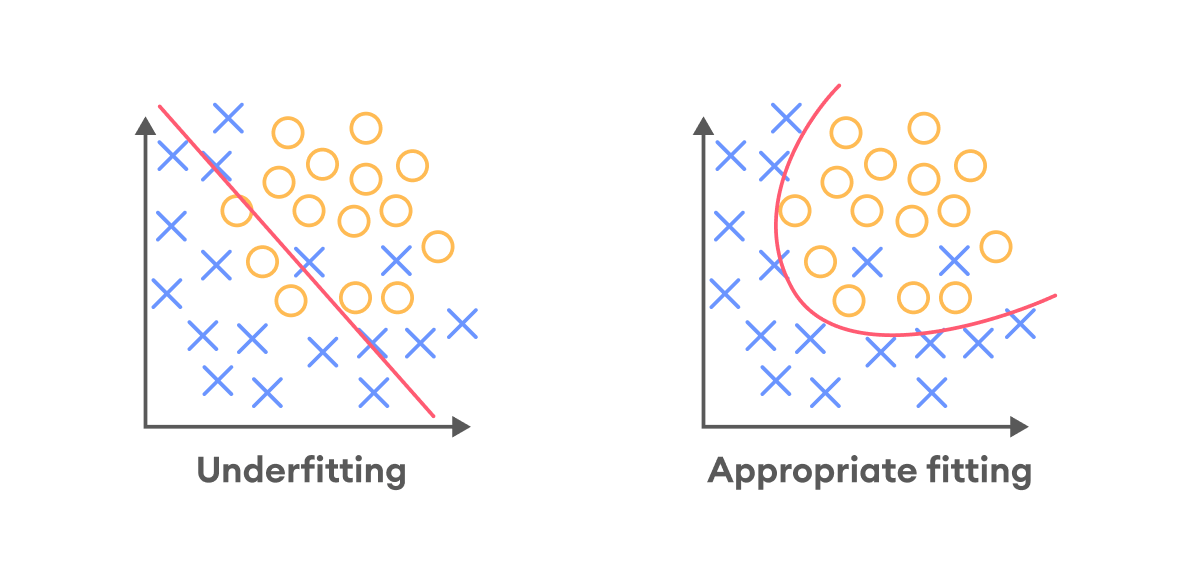
\includegraphics[scale=0.25]{images/03.png}
\end{center}

\begin{itemize}
  \item In the above figure, the left-side model represent  \( h_\w(x) = w_0 + w_1x \) for some \(w_0, w_1\), but it doesn't fit the given dataset well.
  \item Right-side model fits the dataset well, and represents \( h_\w(x) = w_0 + w_1x + w_2x^2 \) for some \(w_0, w_1, w2\).
  \item This suggests we may want to change/transform the feature space we are working with for improved model fits. We detail the procedure below using basis functions.
\end{itemize}

Given a basis function $\phi:\mathcal{X}\rightarrow \mathbb{R}^{m + 1}$, where
\begin{align*}
  \phi(\x) =
  \begin{bmatrix}
    1          \\
    \phi_1(\x) \\
    \phi_2(\x) \\
    \vdots     \\
    \phi_m(\x)
  \end{bmatrix}_{(m + 1)\times 1}
\end{align*}
The hypothesis space becomes
\begin{align*}
  \mathcal{H}_\phi = \left\{\left.h_\mathbf{w} \in \mathcal{X}^\mathbb{R}\right|\mathbf{w}\in\mathbb{R}^{m + 1}, h_\mathbf{w}(\x) = \mathbf{w}^\top\phi(\x)\text{ for }\x \in \mathcal{X}\right\}
\end{align*}

The design matrix with basis function-based transformations can be written as:
\begin{align*}
  \mathbf{\Phi}_\D =
  \begin{bmatrix}
    \phi(\x_1)^\top \\
    \phi(\x_2)^\top \\
    \vdots          \\
    \phi(\x_n)^\top
  \end{bmatrix}_{n\times(m + 1)}
\end{align*}
Note that $\mathbf{\Phi}_\D$ yields $m$-dimensional feature vectors, that could be smaller or larger than the original $d$-dimensional input feature space.

The least-squares objective using basis functions can be written as:
\begin{align*}
  \mathcal{L}_{\text{LS}}(h_\mathbf{w}, \D) & = \dfrac{1}{n}\sum_{i = 1}^n(y_i - h_\mathbf{w}(\x_i))^2           \\
                                            & = \dfrac{1}{n}\sum_{i = 1}^n(y_i - \mathbf{w}^\top\phi(\x_i))^2    \\
                                            & = \dfrac{1}{n}\norm{ \mathbf{y} - \mathbf{\Phi}_\D\mathbf{w} }_2^2
\end{align*}

and as before
\begin{align*}
  \mathbf{w}^*_{\text{LS}} = \left(\mathbf{\Phi}_\D^\top\mathbf{\Phi}_\D\right)^{-1}\mathbf{\Phi}_\D^\top\mathbf{y}
\end{align*}

\newpage
\subsection{Examples of Basis Functions}
\begin{itemize}
  \item \tc{Polynomial Basis}\\ For 1-D data, \(\Phi_j(x) = x^j\) for \(1 \leq j \leq d\) .
  \item \tc{Radial Basis Function(RBF)}\\
        For $d$-dimensional data, \(\Phi_j(\mathbf{x}) = e^{-\frac{\|\mathbf{x}-\mu_j\|_2^2}{\sigma_j^2}}\) for \(\mathbf{x},\mu_j \in \mathbb{R}^d, \sigma_j \in \mathbb{R}\) .
  \item \tc{Fourier Basis}
  \item \tc{Piecewise Linear Basis}
  \item \tc{Periodic Basis ($\sin(x)$, $\cos(x)$ etc.)}
\end{itemize}

\begin{mdframed}
  \tc{Data Splits (Preliminaries)} :
  The original data in a machine learning model is typically taken and split into three sets.
  \begin{itemize}
    \item Training data (Training set): Dataset used to train the model and learn the parameters. (Below, $n$ is the number of data points in the training set)
          \begin{center}$D = \{(\x_i, y_i)\}_{i=1}^n$\end{center}
          \begin{center}Training Error : $\dfrac{\Sigma_{i=1}^n (y_i - h_\w(\x_i))^2}{n}$\end{center}
    \item Development Set (Validation Set) : Mainly used to tune \textit{hyperparameters} of the model. Hyperparameters are not learnable parameters, and are instead predetermined quantities that are used with the model. For example, $\sigma$ in an RBF basis function is a hyperparameter.
    \item Test Set (Evaluation Set) : This is the unseen/test set used for a final evaluation of the model, after choosing the best hyperparameters determined via tuning on the development set. The error on the test set is also referred to as the generalization error.
  \end{itemize}
  Errors on the development/test sets are a measure of the generalization ability of the trained machine learning model.
\end{mdframed}

\section{Hyperparameter tuning}

Hyperparameter tuning involves two general methods :
\begin{itemize}
  \item Grid Search: Define a search space as a grid of hyperparameter values and evaluate every position in the grid.
  \item Random Search: Define a search space as a bounded domain of hyperparameter values and randomly sample points in that domain.
\end{itemize}

\subsection{Underfitting}
Underfitting is a scenario where a data model is overly simple and unable to capture the relationship between the input and output variables accurately.

\begin{figure}[H]
  \centering
  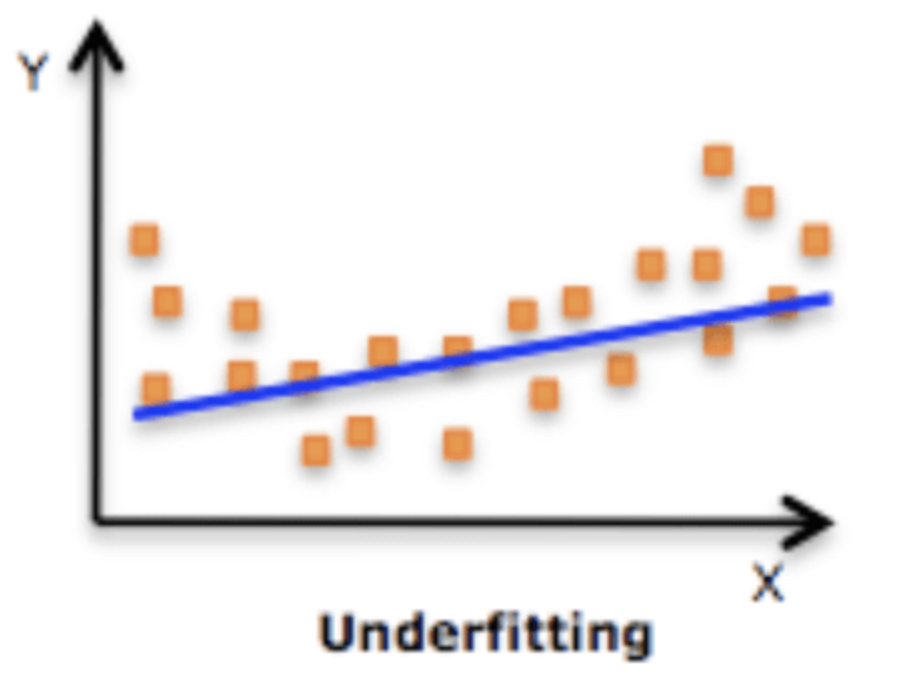
\includegraphics[scale=0.35]{images/04.png}
  \caption{Model is too simple and underfits the data}
\end{figure}

\subsection{Overfitting}
Overfitting is an undesirable machine learning behavior that occurs when the machine learning model gives accurate predictions for training data but not for new data (i.e., does not generalise well). Model fits the training data perfectly but is overly complex.

\begin{figure}
  \begin{subfigure}{0.45\textwidth}
    \centering
    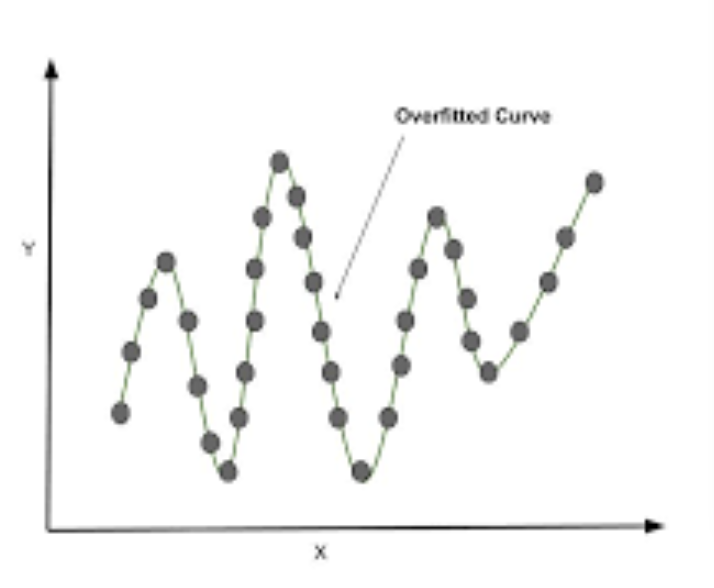
\includegraphics[scale=0.4]{images/05.png}
    \caption{Model is overly complex}
  \end{subfigure}
  \begin{subfigure}{0.45\textwidth}
    \centering
    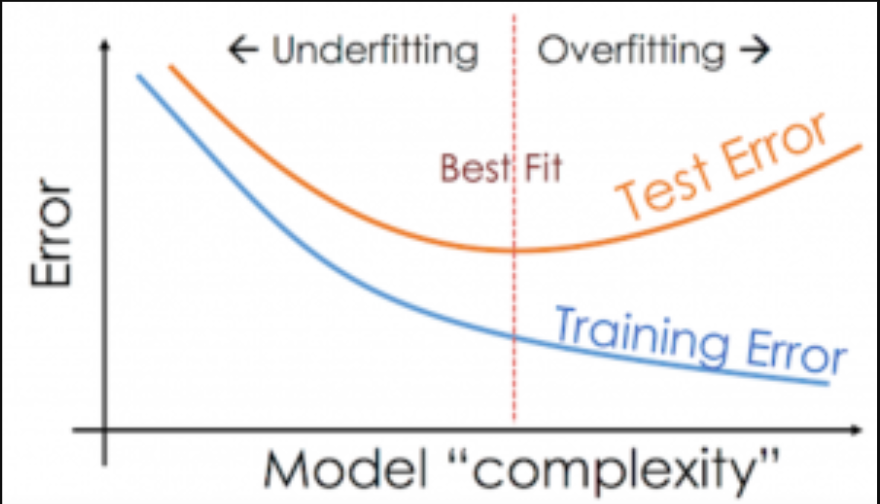
\includegraphics[scale=0.4]{images/06.png}
    \caption{Hyperparameter tuning}
  \end{subfigure}
\end{figure}

It is tempting to assume that having large number of parameters (making complex model) in our hypothesis class would fit the training data perfectly. But this would fail to predict new unseen data miserably. This is termed \tc{overfitting}.

\begin{figure}[H]
  \begin{subfigure}{0.45\textwidth}
    \centering
    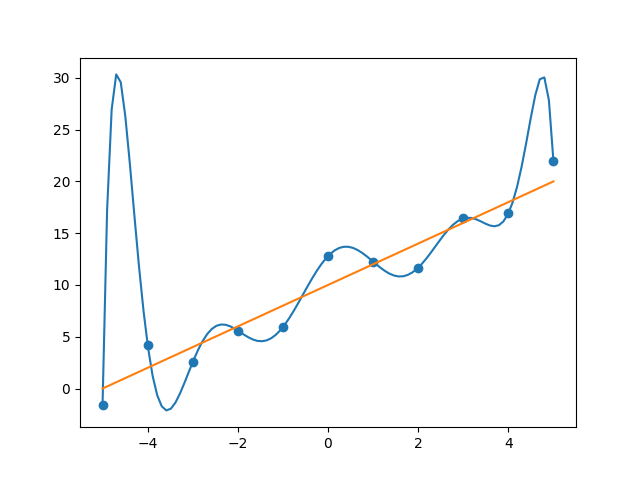
\includegraphics[scale=0.45]{images/07.png}
    \caption{Original}
  \end{subfigure}
  \hfill
  \begin{subfigure}{0.45\textwidth}
    \centering
    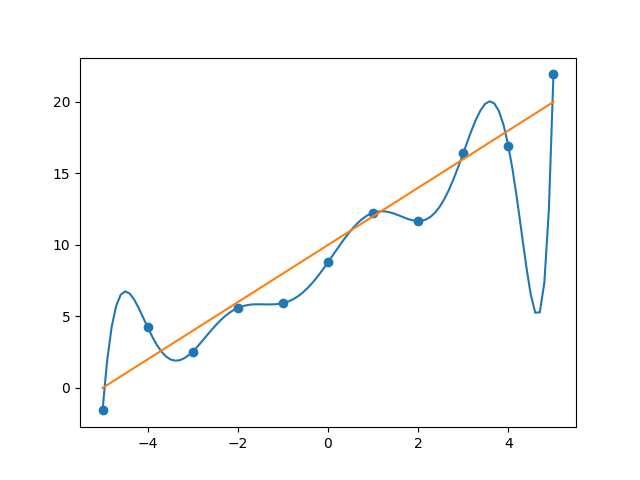
\includegraphics[scale=0.45]{images/08.png}
    \caption{Perturbation}
  \end{subfigure}
  \caption{Overfitting due to complex modelling}
\end{figure}

Consider the line y = 2x+10, let's say we sampled few points from this true line, and this process had some noise involved. In the above figure, we try to fit a polynomial regression model with degree 10. Our predictor function $h_\w(\x)$ is given as:
$$
  h_\w(\x) = w_0 + w_1x + w_2x^2 + \dots + w_{10}x^{10}
$$

It is clearly evident from the image, that the training error is 0, the model perfectly fits the training data, but the test error is fairly high due to the huge variance of the predictor function. Additionally, on small perturbation(here, changing the the data point(0,13) to (0,8) in the second image), has vastly changed the shape of the curve fit, because of several degrees of freedom. \\

Ideally we would want to hit the sweet spot between a simple fit (Underfitting, suffering from high bias) and a complex fit (Overfitting, suffering from high variance), and thus we need to tune the hyperparameter $d$.

\section{Regularization}
Instead of tuning, regularization modifies the loss function to explicitly constrain the model complexity. The general regularised optimisation equation looks like:
$$
  L_{reg}(\w, D_{train}) = L_{MSE}(\w, D_{train}) + \lambda R(\w)
$$

where the first term, $L_{MSE}(\w, D_{train})$ is the measure of fit to the training data set and the second term $\lambda R(\w)$ is the regulariser term, with $\lambda \geq 0$. The $R(\w)$ is a measure of the model's complexity. This can help alleviate overfitting caused by the first term. It does this by penalising/shrinking weights in the weight vector making some of them equal to near zero, Thus even if the model is a high-degree polynomial, minimizing the $L_{reg}$ yields many (near) zero weights, thereby shrinking the model complexity. Two examples of these shrinkage-based regularizations are discussed in the sections below.\\

\fbox{
  \begin{minipage}{\textwidth}
    \tc{Why this works?}
    When the coefficients are very large and the model is highly complex, the errors on dev set or test set are large due to large variances in the predictor function. This can be alleviated by penalising the weight terms(weight norm), thereby making values of $\w$ small, and hence the errors are not every large!
  \end{minipage}
}

\subsection{Ridge Regression}

Ridge regression (also called L2-Normalised Regression) is a regularization technique to combat overfitting. The penalty term $R(\w)$ here is a Euclidean norm, given as $R(\w) = ||\w||^2$. The optimisation objective function and the optimal weights for L2-regularized regression can be written as:
\[ \w_{L_2} = \argmin_\w (||\y-\phi \w||_2^2 + \lambda||\w||_2^2)\]
The above equation is equivalent to the following constrained optimization problem.
\[\w_{L_2} = \argmin_\w ||\y-\phi \w||_2^2 \text{ s.t } ||\w||_2^2 \leq t^2 \]
\fbox{
  \begin{minipage}{\textwidth}
    Note: Usually, we don't include $w_0$ in the penalty term R($\w$). This goes well with the intuition that the intercept doesn't depend on the feature vectors and hence penalising $w_0$ would lead to a poor fit.
  \end{minipage}
}\\

Infact, this optimisation problem has a closed form solution just as the non regularised objective function.
\[\nabla L_{ridge}(\w) = 0\]
\[-2 \phi^T(\y-\phi \w) + 2\lambda \w = 0\]
\[\w_{ridge} = (\phi^T\phi + \lambda I)^{-1} \phi^T\y\]

\fbox{
  \begin{minipage}{\textwidth}
    Note: The best thing about the closed form solution is that such a closed form solution always exists, unlike the unregularized loss function solution, because here the term $\phi^T\phi + \lambda I$ is always invertible(provided the regularization parameter $\lambda > 0$). \\

    A matrix $\X \in \mathbb{R}_{n \times n}$ is positive definite if for any $\tc{v} \neq 0$, $\tc{v}^T\X\tc{v} > 0$. And a positive definite matrix is always invertible. Since $\tc{v}^T\X\tc{v} > 0$ for all $\tc{v} \neq 0$, this implies $\X \tc{v} \neq 0$ for all $\tc{v} \neq 0$, which is the definition of an invertible matrix.\\

    In our case, consider a non zero vector $\tc{v}$,
    $$
      \tc{v}^T(\phi^T\phi + \lambda I) \tc{v} = \tc{v}^T\phi^T\phi \tc{v} + \lambda \tc{v}^T\tc{v} = (\phi \tc{v})^T\phi \tc{v} + \lambda \tc{v}^T \tc{v} = ||\phi \tc{v}||_2^2 + \lambda ||\tc{v}||_2^2
    $$

    The above expression is strictly positive for positive values of $\lambda$.
  \end{minipage}
} \\

\subsection{Lasso Regression}

Also known as L1-normalised regression, Lasso (Least Absolute Shrinkage \& Selection Operation) Regression is a similar technique to Ridge regression, but instead of using Euclidean L2 norm for the penalty, we use the L1 norm. So $R(\w) = ||\w||_1$, and the total loss function can be expressed as:
\begin{equation*}
  \w_{L_1} = \argmin_\w (||\y-\phi \w||_2^2 + \lambda||\w||_1)
\end{equation*}
The equivalent constrained form for the above is:
\begin{equation*}
  \w_{L_1} = \argmin_\w (||\y-\phi \w||_2^2) \text{ s.t } ||\w||_1 \leq t
\end{equation*}
As the L1 norm isn't differentiable, there is no closed form solution for the above optimisation problem. Other methods which can be used to solve for the optimal weights:
\begin{itemize}
  \item Quadratic Programming
  \item Iterative optimisation algorithms (e.g. Gradient Descent)
\end{itemize}

\subsection{Comparison}

L1 Regularization yields sparse weight vectors compared to L2 Regularization. This can be intuitively understood from an example. \\

Referring to the figure below diagram, assume the constrained version of the regularization methods, and the predictor with only two weights $\beta_1$ and $\beta_2$. Say, at $\hat{\beta}$, the MSE is minimised. So around that we draw the contours(ellipses) of the loss function, and the points at which a contour touches the boundary of enclosed area by the constraints (rhombus in Lasso, and circle in Ridge) gives the final optimal weights.\\

There will be a large number of cases, where the contour will touch the square at one of its corners (one weight resulting in zero) as compared to touching the circle on the axes. By extrapolation, we can see that in higher dimensions, the cases where multiple weights are zero will occur much more frequently in Lasso regression due to the sharp boundaries. So Lasso regression will prove to be useful in cases when there are outliers present in the training data and using Ridge regression could result in non-zero weights of undesired features present in the set of basis functions. Lasso can effectively ignore these features by setting their weights to zero. Ridge, with its more gradual constraints, might still assign non-zero weights to these features. \\

\fbox{
  \begin{minipage}{\textwidth}
    \tc{Note}: It is not that always sparsity helps. Infact, for neural networks L2 regularization is most widely used (due to its smoothness). But for many benchmark tasks (feature selection tasks), L1 regularization is preferred and encourages models that utilize a smaller subset of features, which can be valuable for interpretability and reduces computational complexity.
  \end{minipage}
}

\begin{figure}[h]
  \centering
  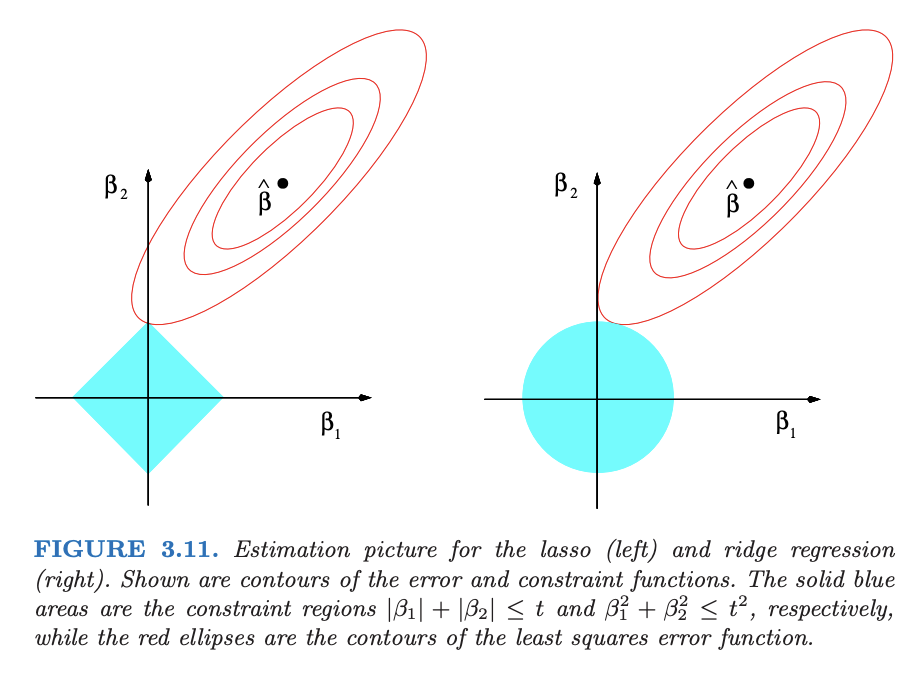
\includegraphics[width=0.7\textwidth]{images/09.png}
  \caption{Comparison of L1 and L2 Regression methods. Figures reproduced from The Elements of Statistical Learning  (Trevor Hastie, Robert Tibshirani and Jerome Friedman. Second Edition. 2009)}
\end{figure}